%!TEX program = xelatex
% 完整编译方法 1 pdflatex -> bibtex -> pdflatex -> pdflatex
% 完整编译方法 2: xelatex -> bibtex -> xelatex -> xelatex
\documentclass[lang=cn,11pt]{elegantpaper}
\usepackage{soul} %是用高亮
\usepackage{subfigure}% 使用子图
\usepackage{setspace}% 使用字体调整
\setcaptionwidth{30em}% 调整caption宽度
\usepackage{multirow}

% \hspace{1em}

\title{雷达引导的小障碍物分割}
\author{共同一作:Aasheesh Singh, Aditya Kamireddypalli, Vineet Gandhi1 和 K Madhava Krishna1  }

\institute{国际信息技术学院, 海德拉巴, 印度}

% 不需要版本信息,直接注释即可
\version{英译汉}
% 不需要时间信息的话,需要把 \today 删除。
\date{International Conference on Intelligent Robots and Systems (IROS 2020) }


% 如果想修改参考文献样式,请把这行注释掉
\usepackage[authoryear]{gbt7714}  % 国标

\begin{document}

\maketitle

\begin{abstract}
\noindent 

检测道路上的小障碍物对自动驾驶来说至关重要。在本文中,我们提出了一种方法,通过稀疏LiDAR(VLP-16)和单目相机的多传感器框架来可靠地检测这些障碍物。LiDAR被用来以置信度图的方式向单目分割网络提供额外的信息。
实验表明,当环境信息被作为额外的维度输入到单目语义分割框架时,性能得到了显著的提高。
我们进一步提出了一个新的语义分割数据集,其中包括3000多个图像帧和相应的LiDAR点云数据\hl{}\footnote{其中有标签的(真正可用的)数据约1600帧。} 。
这些图像带有三个类别的语义分割标签——道路外、无障碍道路和小型障碍物。本文指出LiDAR和相机之间的精确标定对这项任务至关重要,也因此提出了一种基于新型Hausdorff距离的细化外参标定方法。
作为这个数据集的第一个基准,我们的方法在具有挑战性的场景下,50米的距离内障碍物分割准确率达到73\%。从分割质量上看,我们实现了在50米处对低于15厘米高的障碍物进行准确分割;从分割效果的指标上看,我们比现有算法更好,证明了该方法的有效性。我们的代码和数据集存放在 \href{https://small-obstacle-dataset.github.io/}{https://small-obstacle-dataset.github.io/}
\footnote{译者根据其论文复现并修正了其算法,项目地址为:\href{https://github.com/LT1st/SmallObstacleDetection}{https://github.com/LT1st/SmallObstacleDetection}。}。

\keywords{小障碍物检测, 注意力机制, 多传感器融合, 实例分割}
\end{abstract}


\section{介绍}
在自动驾驶的感知算法中,小障碍物检测是一个重要的问题。小障碍物处于被分割为可行驶区域或障碍物的边缘\footnote{表现为此类像素为在两类(障碍物和道路)上置信度都不高。}。谨慎的设计方法要求自动驾驶汽车的路径规划模块能获得环境中小障碍物的信息。
由于小障碍物在整体图像中占比\footnote{此处占比指:远距离小障碍物在像素平面投影量相对于整个图像平面大小,在检测上难。}较小,直接将语义分割方法拓展到小障碍物分割任务,并获得较好的连续分割效果是困难的。
由于这样的小区域类在预测的标签空间中占据了很小的部分\footnote{此处占比指:障碍物和可行驶道路的标签分布数量不均衡,在训练模型(统计学习)上难。},障碍物对应像素的损失函数数值很小,导致训练过程中梯度较小,模型参数更新的量很小。
为了克服这些问题,诸如[5,1]等方法提出了对小区域类标签敏感的成本函数(中值频率平衡),这些方法取得了一定的效果。
然而,这类算法并没有测试路面低矮障碍物的识别情况,而仅展示了远距离识别如电线杆和交通标志这类小障碍物的效果。
因为路面上有低矮障碍物的样本在精挑细选的自动驾驶数据集中十分罕见,所以识别低矮障碍物对感知算法来讲是严峻的挑战\footnote{这里特指监督学习下的算法,缺乏样本就意味着算法性能弱。}。
此外,如果障碍物外观与道路相似,它们更不容易被检出(比如图\ref{fig1}中显示的水泥路面上的石头障碍物)。在本文中,我们开发了另一种模型——将激光雷达和图像输入有效地融合,用于道路小障碍物检测。

\begin{figure}[hp]
\centering

    \subfigure[]
    {
        \begin{minipage}[b]{.3\linewidth}
            \centering
            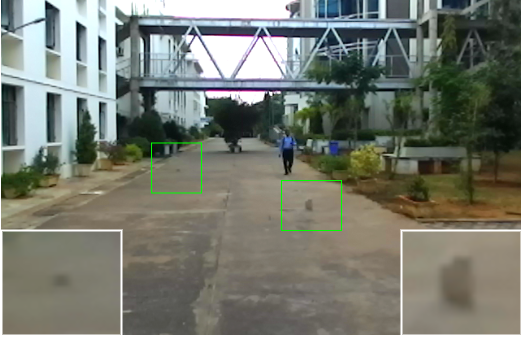
\includegraphics[scale=0.24]{figure/1_a.png}
        \end{minipage}
    }
    \subfigure[]
    {
     	\begin{minipage}[b]{.3\linewidth}
     	
            \centering
            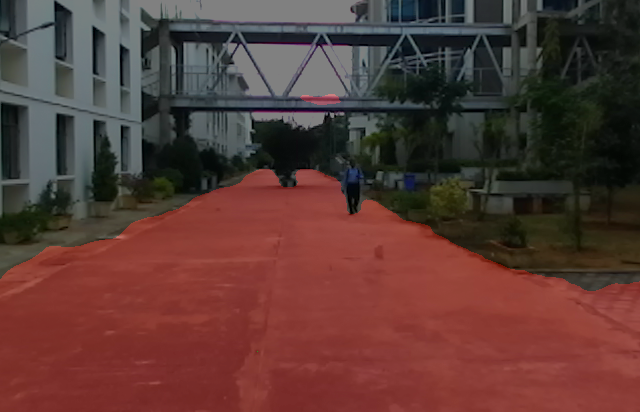
\includegraphics[scale=0.2]{figure/1_b.png}
        \end{minipage}
    }
    \\
    \subfigure[]
    {
     	\begin{minipage}[b]{.3\linewidth}
            \centering
            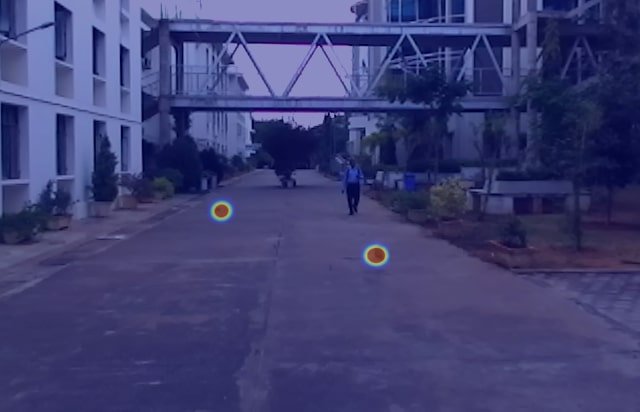
\includegraphics[scale=0.2]{figure/1_c.png}
        \end{minipage}
    }
    \subfigure[]
    {
     	\begin{minipage}[b]{.3\linewidth}
            \centering
            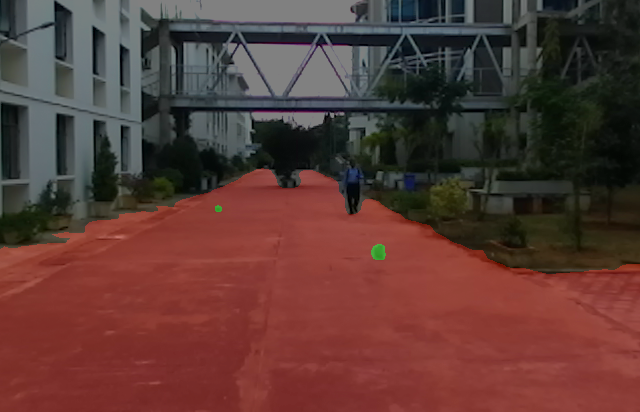
\includegraphics[scale=0.2]{figure/1_d.png}
        \end{minipage}
    }
    \caption{检测样例: (a)原始图像有有两个小障碍物(绿色矩形)。 (b) 单目RGB检测模型未检出两个障碍物。 (c) 使用LiDAR点云生成的背景(置信度图)。 (d) 本文提出的方法(单目与LiDAR结合)成功检测到这两个障碍物。 \label{fig1}}% 不放在这里编译过不了
\end{figure}

在我们的方法中,稀疏的Velodyne Puck 16获得的LiDAR点云,用来通过间断点检测器扫描其中可能的障碍物区域。两个不连续点之间的一组连续的三维点构成了一个可能存在小障碍物的候选区域。这些候选区域通过LiDAR-Camera extrinsics投影到图像平面上,并通过高斯模糊算子进一步模糊化。图像中的这些模糊区域被分配了概率分数,代表了对小障碍物的置信度\footnote{也就是对于图像中的某个像素,它是障碍物这一类别的概率。},因此被称为置信度图。置信图与输入的RGB图像一起构成了四通道输入深度卷积网络(DCNN)。在道路、道路外、小障碍物三个类别的监督下,该网络可以准确地检测出小障碍物区域。而这对于纯图像的分割框架来说是很困难的(图1展示了一个有说服力的例子)。实验表明,通过LiDAR和图像的传感模式的融合,小障碍物区域的检测和分类精度比仅基于图像的网络有了显著提高。
总之,我们的论文有以下贡献:

1. 一个新的LiDAR-Camera小障碍物分割数据集(表\ref{tab:dataset}),包括3000多帧,每像素注释道路、道路外和小障碍物3个类别,以及LiDAR-Camera校准外参。这个数据集也可以作为纯图像或纯激光雷达的小障碍物分割数据集。  

\begin{table}[h]
\centering
\caption{小障碍物数据集描述}
\begin{tabular}{|l|c|c|c|c|}
\hline
\textbf{划分} & \textbf{\# 录像数} & \textbf{\# 图像数} & \textbf{有路牙} & \textbf{无路牙} \\

\hline\hline
     \textit{Train} & 9 & 1937 & 6 & 3\\
     \textit{Validation} & 4 & 530 & 2 & 2\\ 
     \textit{Test} & 2 & 460 & 1 & 1\\
     \hline\hline
     \textbf{总计} & $\mathbf{15}$ & $\mathbf{2927}$ & 9 & 6\\
\hline
\end{tabular}

\label{tab:dataset}
\end{table}

2. 一个新颖的算法,将LiDAR点云中获得的置信图与RGB通道\footnote{此处的RGB指单目相机的数据,区分与置信度图拼合后的RGBA四通道图像。}相结合作为输入,获得了比纯图像架构(如[2, 18])更显著的提升。值得注意的是,稀疏的LiDAR扫描可能会完全错过小的障碍物,因此,仅仅依靠当前帧的LiDAR输入是不严谨的。可以通过将先前帧的LiDAR置信图传播到当前帧来克服这个问题,这样,即使本次LiDAR扫描完全错过小障碍物,先前帧的障碍物检测也可以提供置信度图。我们在V-B节中描述了这些结果。这项工作的另一个重要贡献是,使用稀疏的Puck 16 LiDAR更适合于点云分割,而不是采样更密集的64线LiDAR。

3. 对构成整体算法的LiDAR-Camera校准、置信图的生成、置信图时序传播等模块,进行了详细的消融实验。

4. 一种新的基于Haussdorf距离的无标记LiDAR-Camera标定方法。由于提升了外参精度,大幅改善了训练时间和准确性。

5. 最后,与大多数只在图像或密集的点云数据上运行的分割方法不同,这是已知的第一个将稀疏的LiDAR数据与单目图像融合来分割小障碍物的方法。

\begin{figure}[hp]
    \centering
    % \captionsetup{font={small,stretch=1.25}, justification=raggedright}
    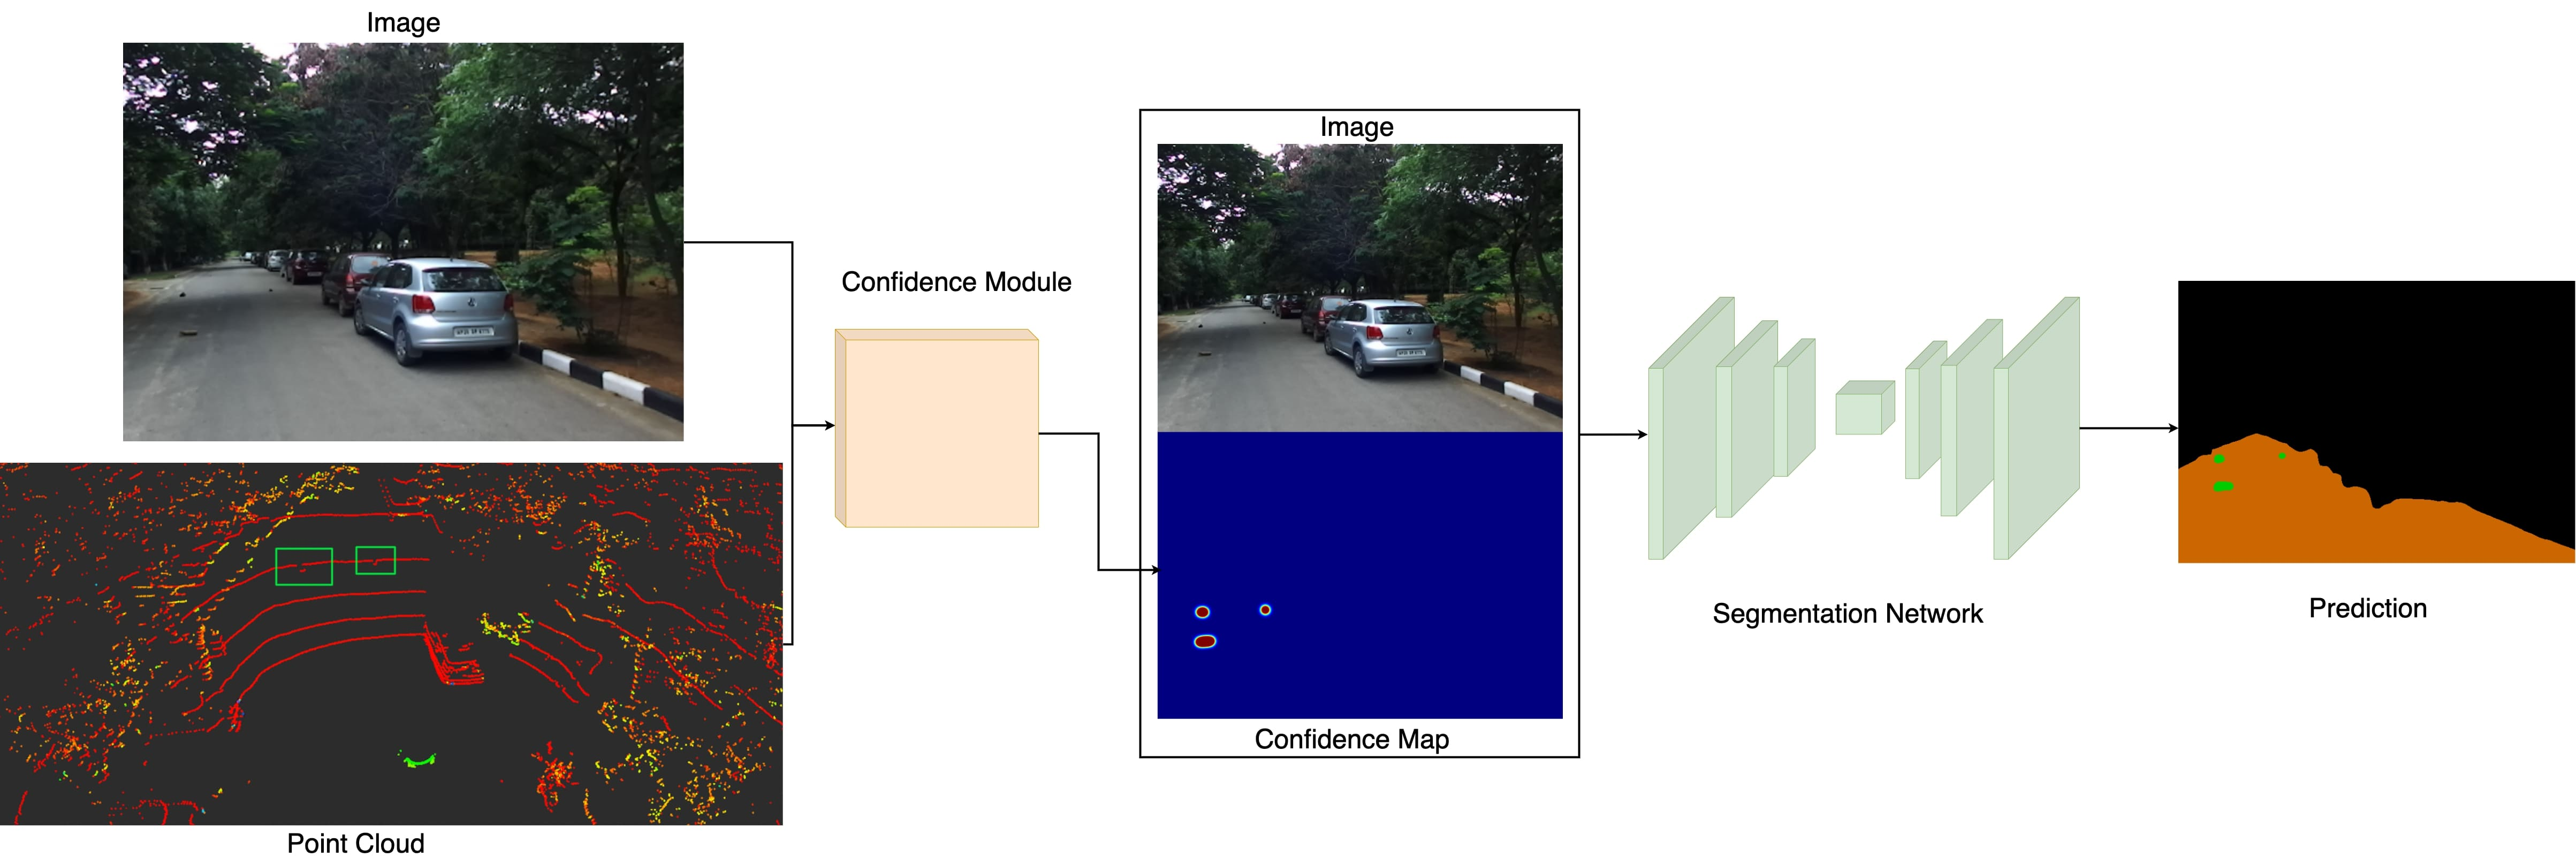
\includegraphics [ width =0.7 \textwidth ]{ ./figure/2.png}
    \caption { 本文提出的小障碍物检测流程。置信模块根据点云生成一个置信图。该结果与当前图像相拼接,并用于预测分割掩码。 \label { fig : 2 }}
\end {figure}


\section{结论}
我们的工作着眼于融合单目RGB和LiDAR数据来检测道路上的小障碍物。我们的实验表明,当一个给定的纯图像RGB分割网络被LiDAR提供的置信图所增强后,IDR指标增加了40-50\%。使用两个SOTA网络DeepLAB V3+和HRNet进行的详细实验证明了本文的方法的有效性(表\ref{tab:results})。我们还提出,可以利用小障碍物的真实标签来改善外参标定效果,这反过来又改善了IDR指标(表\ref{tab:5})。

我们进一步提出了详细的消融实验,以证明设计选择的合理性。总之,我们的方法能够检测到50米范围内73\%的小障碍物(15厘米高)。



\begin{figure}[h]%%参数: h:放在此处 t:放在顶端 b:放在底端 p:在本页
    \centering
    % \captionsetup{font={small,stretch=1.25}, justification=raggedright}
    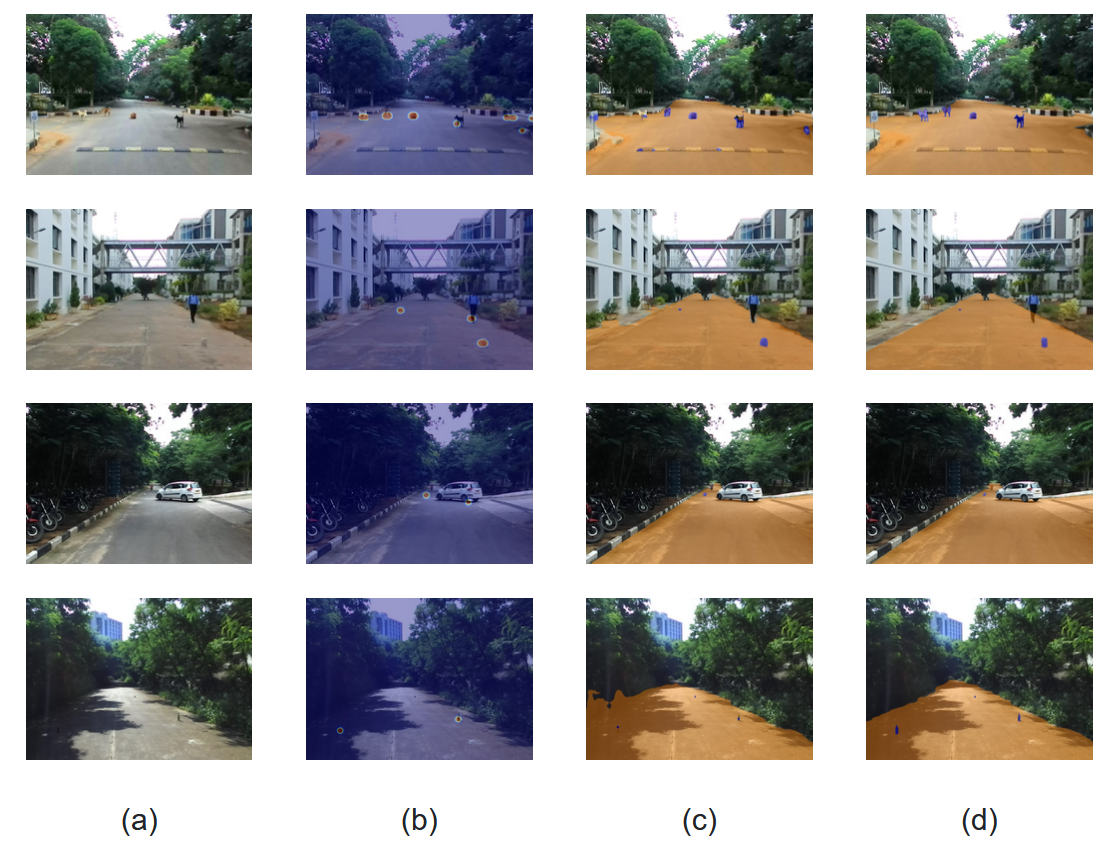
\includegraphics [ width =0.7 \textwidth ]{ ./figure/7.png}
    \caption { (a) RGB原图图像。(b) 置信度图 (c) 分割结果。(d)真实标签。 \label { fig : 7 }}
\end {figure}

\begin{table}
\centering
\caption{语义分割架构的各种输入的性能比较}
\begin{tabular}{|l|l|c|c|c|c|}
\hline
\multirow{2}{*}{\textbf{Network}} & \multirow{2}{*}{\textbf{Method}} & \multicolumn{2}{|c|}{\textbf{Instance-level}} & \multicolumn{2}{|c|}{\textbf{Pixel-level}}\\

& & IDR & iFDR & PDR & mIoU \\

\hline\hline
     \multirow{3}{5em}{\textbf{DeepLab-V3+}\cite{DeepLab}} & \textit{Image} &  0.39 & 0.28 & 0.37 & 0.73\\
     & \textit{Image + CM} & 0.50 & 0.26 & 0.45 & 0.74\\ 
     & \textit{Image + CM + TP} & \textbf{0.60} & \textbf{0.18} & \textbf{0.60} & \textbf{0.76}\\
     
\hline
    \multirow{3}{5em}{\textbf{HRNet}\cite{HRNet}} & \textit{Image} &  0.44 & 0.25 & 0.27 & 0.70\\
     & \textit{Image + CM} & 0.47 & 0.25 & 0.32 & 0.70\\
     & \textit{Image + CM + TP} & \textbf{0.63} & \textbf{0.21} & \textbf{0.51} & \textbf{0.73}\\ 
\hline
\end{tabular}

\label{tab:results}
\end{table}



\begin{table}[h]%%参数: h:放在此处 t:放在顶端 b:放在底端 p:在本页
  \small
  \centering
  \caption{粗校和精校之间的检测性能比较。  }
  \label{tab:5}
  
    \begin{tabular}{l|c|c c c}
    \toprule
           外参    &   $\sigma$  &   IDR & iFDR & PDR     \\
    \midrule% 表中线
    先Hausdorff标定   &    5     &   0.412 &  0.263 & 0.363   \\
        &    7     &   0.412 &  0.263 & 0.363   \\
    后Hausdorff标定    &  5 & 0.50 & 0.26 &  0.45 \\
        &  7       & 0.50 & 0.26 &  0.45 \\
    
    \bottomrule% 表底线
    \multicolumn{5}{l}{\scriptsize $\sigma$表示高斯模糊的方差参数} \\
    \end{tabular}%
\end{table}%

指标计算公式如下:
\begin{equation}
    \mathit{IDR} = \frac{TP_{obstacle}}{TI_{obstacle}}
\end{equation}
\begin{equation}
    \mathit{iFDR} = \frac{FP_{obstacle}}{PRED_{obstacle}}
\end{equation}
\begin{equation}
    \mathit{PDR_{obstacle}} = \frac{TPX_{obstacle}}{GTX_{obstacle}}
\end{equation}


\section{论文信息}

作者:Aasheesh Singh, Aditya Kamireddypalli, Vineet Gandhi1 和 K Madhava Krishna1

单位:国际信息技术学院, 海德拉巴, 印度

杂志:International Conference on Intelligent Robots and Systems (IROS 2020 \footnote{IROS是机器人领域顶会:\href{http://robot.buaa.edu.cn/info/1024/1047.htm}{机器人领域SCI期刊及重要国际会议}})


日期:2020年3月12日

检索号:  

\quad 1. DOI: 10.1109/IROS45743.2020.9341465   

\quad 2. Print on Demand(PoD) ISBN:978-1-7281-6213-3  

\quad 3. Electronic ISBN:978-1-7281-6212-6   

\quad 4. INSPEC Accession Number: 20424760

被引次数: 3



\nocite{*}

% 如果想修改参考文献样式(非国标),请把下行取消注释,并换成合适的样式(比如 unsrt,plain 样式)。
%\bibliographystyle{aer}
% \bibliography{wpref}% 控制是否显示引文

\end{document}
